\documentclass[journal]{IEEEtran}
\usepackage[a5paper, margin=10mm]{geometry}
%\usepackage{lmodern} % Ensure lmodern is loaded for pdflatex
\usepackage{tfrupee} % Include tfrupee package


\setlength{\headheight}{1cm} % Set the height of the header box
\setlength{\headsep}{0mm}     % Set the distance between the header box and the top of the text


%\usepackage[a5paper, top=10mm, bottom=10mm, left=10mm, right=10mm]{geometry}

%
\usepackage{gvv-book}
\usepackage{gvv}
\setlength{\intextsep}{10pt} % Space between text and floats

\makeindex

\begin{document}
\bibliographystyle{IEEEtran}
\onecolumn
\newpage
\title{ '2014-EE-'40-52'}
\author{AI24BTECH11004-Bheri Sai Likith Reddy}
\maketitle
\section{SECTION-A}

\begin{enumerate}
       \item In the figure, the value of resistor R is (25 + I/2) ohms, where I is the current in amperes. The
       current I is  \rule{1cm}{0.15mm}
		\begin{figure}[h!]
            \centering
            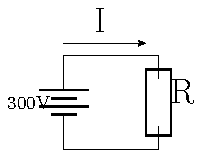
\includegraphics[width=0.2\linewidth]{fig/fig1.pdf}
        \end{figure} \\

	\item In an unbalanced three phase system, phase current $I_\alpha=1\angle \brak{-90^{\circ}}$ pu, negative sequence current $I_(b_2)=4\angle \brak{150_{\circ}}$ pu, zero sequence current $I_c0=3 \angle 90_{\circ}$ pu. The magnitude of phase current $I_b$ in pu is

               \begin{enumerate}
			        \begin{multicols}{4}  
		       \item $1.00$
		       \item $7.81$
		       \item $11.53$
		       \item $13.00$
                    \end{multicols}   
	       \end{enumerate}	
       \item The following four vector fields are given in Cartesian co-ordinate system. The vector field which
does not satisfy the property of magnetic flux density is
		\begin{enumerate}
			\item $y^2a_x+z^2a_x+x^2a_z$
			\item $z^2a_x+x^2a_y+y^2a_z$
			\item $x^2a_x+y^2a_y+z^2a_z$
			\item $y^2z^2a_x+x^2z^2a_y+x^2y^2a_z$
		\end{enumerate}
	\item  The function shown in the figure can be represented as
		\begin{figure}[h!]
            \centering
            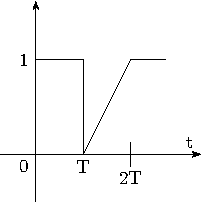
\includegraphics[width=0.3\linewidth]{fig/fig2.pdf}
        \end{figure}

		\begin{enumerate}
			\item $u\brak{t}-u\brak{t-T}+\frac{t-T}{T}u\brak{t-T}-\frac{tu-2T}{T}u\brak{t-2T}$
			\item $u\brak{t}+ \frac{t}{T}u\brak{t-T}-\frac{t}{T}u{t-2T}$
			\item $u\brak{t}-u\brak{t-T}+\frac{t-T}{T}u\brak{t}-\frac{t-2T}{T}u\brak{t}$
	        \item $u\brak{t}+\frac{t-T}{T}u\brak{t-T}-\frac{tu-2T}{T}u\brak{t-2T}$
        	\end{enumerate}
	\item Let $X\brak{z}=\frac{1}{1-z^{-3}}$ be the $Z$-transform of a causal signal $x\sbrak{n}$. Then, the values of $x\sbrak{2}$ and $x\sbrak{3}$ are
		\begin{enumerate}
		       \item $0$ and $0$
		       \item $0$ and $1$
		       \item $1$ and $0$
		       \item $1$ and $1$
        	\end{enumerate}	
	\item Let $f\brak{t}$ be a continuous time signal and let $F\brak{w}$ be its Fourier Transform defined by
 \begin{align*}
     F\brak{w}=\int_{-\infty}^{\infty}f\brak{t}e^{-jwt}dt
 \end{align*}
 Define $g\brak{t}$
 \begin{align*}
     g\brak{w}=\int_{-\infty}^{\infty}F\brak{u}e^{-jut}du
 \end{align*}
 What is the relationship between $f\brak{t}$ and $g\brak{t}$?
		\begin{enumerate}
			\item $g\brak{t}$ would always be proportional to $f\brak{t}$
			\item $g\brak{t}$ would be proportional to $f\brak{t}$ if $f\brak{t}$ is an even function.
			\item $g\brak{t}$ would be proportional to $f\brak{t}$ only if $f\brak{t}$ is a sinusoidal function.
			\item $g\brak{t}$ would never be proportional to $f\brak{t}$
        	\end{enumerate}
	\item The core loss of a single phase, $230/115 V$, $50 Hz$ power transformer is measured from $230 V$ side
by feeding the primary ($230 V$ side) from a variable voltage variable frequency source while
keeping the secondary open circuited. The core loss is measured to be $1050 W$ for $230 V$, $50 Hz$
input. The core loss is again measured to be $500 W$ for $138 V$, $30 Hz$ input. The hysteresis and eddy
current losses of the transformer for $230 V$, $50 Hz$ input are respectively,
		\begin{enumerate}
		       \item $508 W$ and $542 W$. 
		       \item $468 W$ and $582 W$.
		       \item $498 W$ and $552 W$. 
		       \item $488 W$ and $562 W$.
        	\end{enumerate}	
	\item A $15 kW$, $230 V$ dc shunt motor has armature circuit resistance of $0.4 \omega$ and field circuit resistance
of $230 \omega$. At no load and rated voltage, the motor runs at $1400 rpm$ and the line current drawn by
the motor is $5 A$. At full load, the motor draws a line current of $70 A$. Neglect armature reaction.
The full load speed of the motor in rpm is \rule{1cm}{0.15mm}
    
	\item  A $3$ phase, $50 Hz$, six pole induction motor has a rotor resistance of $0.1 \omega$ and reactance of $0.92\omega$.
Neglect the voltage drop in stator and assume that the rotor resistance is constant. Given that the
full load slip is $3\%$, the ratio of maximum torque to full load torque is 
		\begin{enumerate}
            \begin{multicols}{4}
			\item $1.567$
			\item $ 1.712$
			\item $ 1.948$
			\item $ 2.134$
   \end{multicols}
        	\end{enumerate}	
	\item A three phase synchronous generator is to be connected to the infinite bus. The lamps are connected
as shown in the figure for the synchronization. The phase sequence of bus voltage is R-Y-B and
that of incoming generator voltage is R'-Y'-B'.

\begin{figure}[h!]
            \centering
            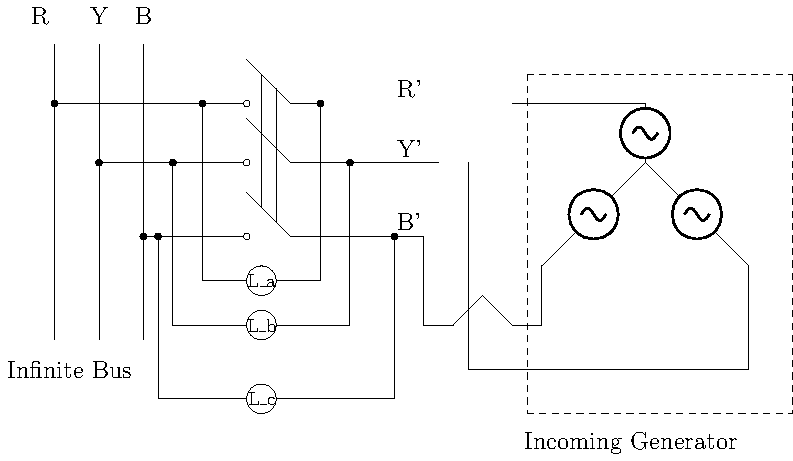
\includegraphics[width=0.5\linewidth]{fig/fig3.pdf}
        \end{figure}
It was found that the lamps are becoming dark in the sequence $L_a -Lb -L_c$ . It means that the phase
sequence of incoming generator is
                \begin{enumerate}
                
			\item opposite to infinite bus and its frequency is more than infinite bus
			\item opposite to infinite bus but its frequency is less than infinite bus
			\item same as infinite bus and its frequency is more than infinite bus
			\item same as infinite bus and its frequency is less than infinite bus
        	
         \end{enumerate}		
	\item  A distribution feeder of $1$ km length having resistance, but negligible reactance, is fed from both the
ends by $400V$, $50 Hz$ balanced sources. Both voltage sources $S_1$ and $S_2$ are in phase. The feeder
supplies concentrated loads of unity power factor as shown in the figure.
\begin{figure}[h!]
            \centering
            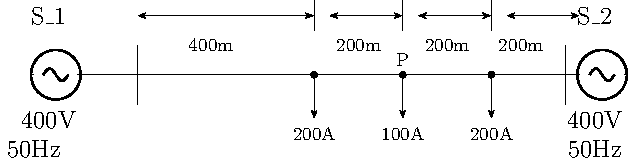
\includegraphics[width=0.5\linewidth]{fig/fig4.pdf}
        \end{figure}
The contributions of $S_1$ and $S_2$ in $100 A$ current supplied at location P respectively, are
		\begin{enumerate}
			\item $75 A$ and $25 A$
			\item $0 A$ and $50 A$
			\item $5 A$ and $75 A$
			\item$ 0A$ and $100A$
        	\end{enumerate}	
	\item A two bus power system shown in the figure supplies load of $1.0+j0.5$ p.u.
		\begin{figure}[h!]
            \centering
            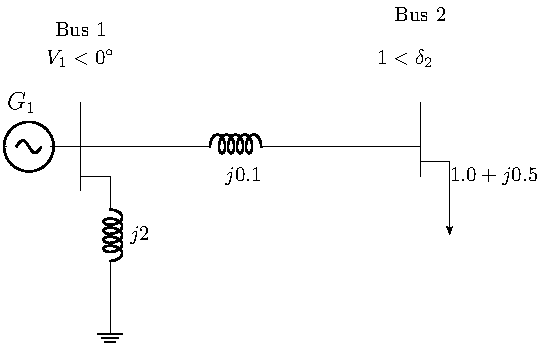
\includegraphics[width=0.5\linewidth]{fig/fig5.pdf}
        \end{figure}
 The values of $V_1$ is p.u. and $\delta ^2$ respectively are
		\begin{enumerate}
			\item $0.95$ and $6.00^{\circ}$
			\item $1.05$ and $-5.44^{\circ}$
			\item $1.1$ and $-6.00^{\circ}$
			\item $1.1$ and $-27.12^{\circ}$
        	\end{enumerate}	
    \item The fuel cost functions of two power plants are 
    \begin{center}
          Plant $P_1$    $C_1=0.05Pg_1^2+APg_1+B$\\
         Plant $P_2$    $C_2=0.10Pg_2^2+3APg_2+B$\\
    \end{center}
    where. $P_{g1}$ and $P_{g2}$ are the generated powers of two plants, and A and B are the constants. If the two plants optimally share $1000 MW$ load at incremental fuel cost of $100Rs/MWh$, the ratio of load shared by plants$P_1$ and $P_2$ is
    
		\begin{enumerate}
			\item $1:4$
			\item $2:3$
			\item $3:2$
			\item $4:1$
        	\end{enumerate}	
\end{enumerate}	
\end{document}

